\section{Finite-radius results on the tuned branches}

The inherited coordinates satisfy the fixed-$\alpha$, fixed-$c$ stationary equations on reevaluation. At $\epsilon=0.01$ for $f_-$,
\begin{equation}
 (R,h_d,h_u)=(1.2781645588,\ 0.2091273511,\ 0.1943861736),\quad
 f=0.2113849121,
\end{equation}
and $\partial_A f=(0.30550539,-0.00384452,-0.00268081)$ on the neutral slice. Its two kinetic matrices are
\begin{align}
 \GJ_{(R,d,u)}&=\JordanMatrix,\\[2pt]
 \GE_{(R,d,u)}&=\EinsteinMatrix.
\end{align}
Thus the conformal completion changes $G_{RR}$ from $-0.3059242$ to $+0.3563763$, and reverses the signs of the displayed radion-amplitude cross terms. The eigenvalues of this Einstein submatrix are approximately $(0.0436681,0.0581720,0.3564345)$. The off-diagonal terms cannot be discarded before computing \eqref{eq:modes}.

\begin{center}
\small\resizebox{\linewidth}{!}{\BranchTable}
\end{center}
All four $m^2$ columns are divided by $\Lam^2$ and are parameters of the two-derivative action. $m_C^2$ is the doubly degenerate charged value; $m_1^2,m_2^2$ are the neutral scalar-dominated values; $m_r^2$ is the radion-dominated value. Four gauge zeros are omitted from the table. The plus/minus differences are numerical profile dependence, not comparisons with measured masses.

At $h=0$, both profiles have $f=0.212145065817\ldots$, as imposed by the earlier common-gravity construction. They need not have identical $f_A$ or kinetic matrices. For $f_-$, the unbroken values are $G^J_{RR}=-0.3071931893$ and $G^E_{RR}=0.3564111501$. At the broken $\epsilon=0.01$ fixture, the plus-minus radion squared-parameter difference is $-1.15870\times10^{-5}$; at $10^{-4}$ it is $-1.15476\times10^{-5}$. Matching the unbroken gravitational coefficient does not eliminate dynamical profile dependence.

To quantify mode identity without reading a coordinate-dependent eigenvector entry, define the normalized projection onto the metric-normal to constant-$R$ slices:
\begin{equation}
 p_{R,\alpha}=\frac{(u_\alpha^R)^2}{((\GE)^{-1})^{RR}},\qquad
 \sum_{\alpha=1}^3p_{R,\alpha}=1.
\end{equation}
On the minus branch, the heavy mode has $p_R=0.99995753$ at $\epsilon=0.01$ and $0.999999676$ at $10^{-4}$. Kinetic and potential mixing are small but included. This is not a gauge-independent particle interpretation beyond the retained effective action.

\subsection{All scalar tangents, charged curvature, and gauge zeros}

The implementation includes all eight real scalar coordinates, not only the two neutral amplitudes. The order is
\begin{equation}
 (R,\operatorname{Re}d_N,\operatorname{Re}u_N,
 \operatorname{Im}d_N,\operatorname{Im}u_N,
 \operatorname{Re}d_C,\operatorname{Re}u_C,
 \operatorname{Im}d_C,\operatorname{Im}u_C).
\end{equation}
Here $u$ denotes the conjugate-up insertion coordinates of the internal operator. This is an invertible real-coordinate choice. At a real neutral background, the matrices separate into the neutral amplitude/radius block, a phase block, and two charged blocks by electric charge and CP. The real charged and phase kinetic blocks for $\epsilon=0.01$, $f_-$ are
\begin{equation}
 \GE_{\rm phase}=\PhaseMatrix,\qquad
 \GE_{\rm charged,Re}=\ChargedMatrix.
\end{equation}
The imaginary charged block has the same spectrum. The eigenvalues of the full nine-dimensional Einstein metric lie between $0.0436681$ and $0.3564345$ for this fixture. Every fixture passes positivity of the full matrix. The potential Hessian has five positive eigenvalues and four symmetry zeros; apparent residual negative values of order $10^{-12}$ are numerical symmetry errors, not resolved negative curvature.

As an additional check, the neutral phase charge tangents for generators $(J_3,Y,X)$ are
\begin{equation}
 C=\begin{pmatrix}-h_d/2&h_d/2&h_d\\h_u/2&-h_u/2&h_u\end{pmatrix}.
\end{equation}
The Higgs contribution to the neutral vector mass matrix obtained independently from the full spectral gauge response equals $C^T\GE_{\rm phase}C$. This low-momentum Ward-identity check also preserves the photon null direction $(1,1,0)$. It does not derive the axion sector or the complete charged-vector kinetic response.

With no axion, the four potential zeros are gauge-orbit tangents. Add the inherited potential-free axion with a positive kinetic coefficient and a pure-$X$ Stueckelberg coupling, with no extra independent derivative mixing. The total scalar-plus-radion-plus-axion system then has ten real directions. Four gauge directions are removed, leaving five positive mass parameters and one massless physical phase. Positivity of the assumed axion coefficient is an input; no numerical axion mass, decay constant, or anomaly completion is inferred. The flat phase prevents a strict isolated minimum even in this restricted description.

\section{Why this does not yet establish full dynamical stability}

The heavy two-derivative parameter is $m_r/\Lam\simeq0.91082$ at $\epsilon=0.01$ and $0.91255$ at $10^{-4}$ for $f_-$. It is about $1.16$ times the first uncoupled spectator fermion scale $\Lam/R$. This is a scale comparison, not an omitted-bosonic-spectrum calculation. There is no demonstrated separation that would justify interpreting the heavy eigenvalue as a pole of the full theory after integrating out everything else.

The exact external-momentum heat integrals contain $e^{-as(1-s)q^2}$. A simple expansion parameter is $a_{\max}|q^2|/4$. Evaluated at the heavy squared parameter it is approximately $1.10$, whereas the larger light neutral value gives $0.0267$ at $\epsilon=0.01$ and $0.000265$ at $10^{-4}$. These numbers diagnose a missing hierarchy; they are not error bounds for a physical propagator.

\begin{figure}[ht]
 \centering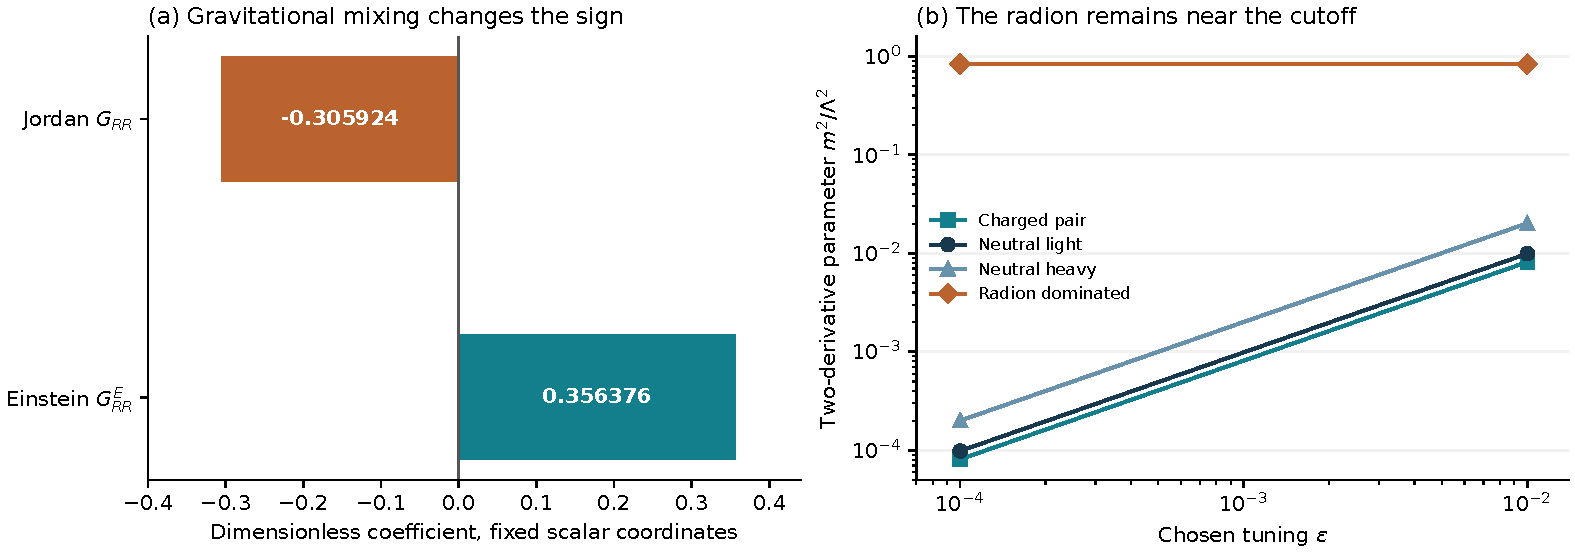
\includegraphics[width=\linewidth]{images/kinetics_and_scales.pdf}
 \caption{Minus-profile diagnostics. (a) Jordan and Einstein radial entries at $\epsilon=0.01$, with all scalar coordinates fixed. Physical scalar positivity uses the full Einstein matrix. (b) Generalized squared-mass parameters of the two-derivative action. The radion remains near the spectral cutoff as the scalar tuning decreases. Lines connect the two computed fixtures; they are not an independently sampled branch.}
\end{figure}

A further check evaluates the full scalar/radius two-point kernel on a \emph{fixed flat Jordan metric}. Writing $z=p_E^2/\Lam^2$, its change from zero momentum is
\begin{multline}
 \Pi_{AB}(z)-\Pi_{AB}(0)=\frac1{8\pi^2}\sum_{a,s}w_an_s
 \operatorname{Re}\sum_{ij}\int_0^1\!\dd t\,e^{-a[tb_i^2+(1-t)b_j^2]}\\
 \times\left[z e^{-at(1-t)z}(T_A)_{ij}(T_B)_{ji}
 +(e^{-at(1-t)z}-1)(A_A)_{ij}(A_B)_{ji}\right].
 \label{eq:momentum}
\end{multline}
Its derivative at zero is \eqref{eq:GJ}. At positive Euclidean $z=0.8295963$, the neutral-amplitude submatrix of $[\Pi(z)-\Pi(0)]/z$ differs in norm from its zero-momentum value by $22.6\%$. The radial entry differs by about $1.14\%$. The large cancellation between Jordan and metric-induced terms means that neither number estimates the physical radion pole shift. The omitted momentum-dependent metric response and Lorentzian continuation are required for that calculation. The full spectral action can have very different ultraviolet behavior from a finite derivative expansion \cite{spectral}.
